\section{Sucesiones}

\begin{questions}

\question
Analice la siguiente secuencia y encuentre la ley que se da en ella:

\[ 0, 3, 8, 15, 24, \ldots \]

De acuerdo con la ley que se da en la secuencia anterior, ¿cuál es el número correspondiente a la posición 11? \footnote{\cite{practicaUCR1}}
\begin{choices}
    \choice  99
    \choice  120
    \choice  132
    \choice  143 
\end{choices}

\begin{solution}
    Una estrategia usual para encontrar patrones es calcular las diferencias entre términos consecutivos y ver si estas tienen un patrón más sencillo. Para que sea más fácil después referirnos a ellos, digamos que el término $n$-ésimo de la sucesión es $T_n$:
    \[
    0 \xrightarrow{+3} 3 \xrightarrow{+5} 8 \xrightarrow{+7} 15 \xrightarrow{+9} 24 \xrightarrow{\phantom{+9}} \cdots
    \]
    Las diferencias son los números impares, por lo tanto, podemos calcular que a 24 hay que sumarle 11, luego a este se le suma 13, etc. Completamos la secuencia hasta la posición 11:
    \[
    0 \xrightarrow{+3} 3 \xrightarrow{+5} 8 \xrightarrow{+7} 15 \xrightarrow{+9} 24 \xrightarrow{+11} 35 \xrightarrow{+13} 48 \xrightarrow{+15} 63 \xrightarrow{+17} 80 \xrightarrow{+19} 99 \xrightarrow{+21} 120
    \]
    Así que el número correspondiente a la posición 11 es $T_{11}=120$, la opción B.

    Con un poco más de experiencia, reconocemos este patrón (el de sumar impares entre términos consecutivos) como el patrón de diferencias entre los números cuadrados perfectos:
    \begin{gather*}
    1 \xrightarrow{+3} 4 \xrightarrow{+5} 9 \xrightarrow{+7} 16 \xrightarrow{+9} 25 \xrightarrow{+11} 36 \xrightarrow{+13} 49\\
    1^2 \xrightarrow{+3} 2^2 \xrightarrow{+5} 3^2 \xrightarrow{+7} 4^2 \xrightarrow{+9} 5^2 \xrightarrow{+11} 6^2 \xrightarrow{+13}7^2
    \end{gather*}
    \vspace{-1cm}
    \shorthandoff{<>}
    \begin{center}
    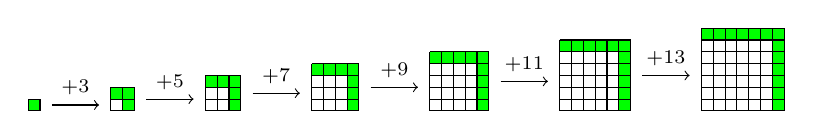
\begin{tikzpicture}[scale=0.15]
        \fill[fill=green] (63,0) rectangle +(7,7);
        \fill[white] (63,0) rectangle +(6,6);
        \draw (63,0) grid +(7,7);
        \foreach \x [evaluate=\x as \y using int(2*\x+1)] in {6, 5, ..., 1} {
            \fill[green] (\x*\x/2+\x/2+5*\x,0) rectangle +(\x, \x);
            \fill[white] (\x*\x/2+\x/2+5*\x,0) rectangle +(\x-1, \x-1);
            \draw (\x*\x/2+\x/2+5*\x,0) grid +(\x, \x);
            \draw[->] (\x*\x/2+\x/2+6*\x+1, \x/2) -- node[above] {$\scriptstyle+\y$} +(4, 0);
        }
    \end{tikzpicture}
    \end{center}
    Por lo que comparando ambas sucesiones, vemos que en la del ejercicio cada término es el cuadrado perfecto asociado a su posición menos uno:
    \begin{align*}
    0 = 1&^2-1,& 3 = 2&^2-1, & 8 = 3&^2-1, &15 = 4&^2 -1,& \dots \\
     &T_1 & &T_2 & &T_3 & &T_4 & \dots
    \end{align*}        

    Por lo tanto, podemos afirmar que el término en la posición $n$ es $n^2-1$. En particular, el término en la posición 11 es $T_{11}=11^2-1 = 121-1 = 120$. Este método nos sirve más cuando el término que se pide está en una posición grande, pues entonces es muy lento ir haciendo las sumas una por una. \hfill $\square$
\end{solution}


\question
Analice la siguiente secuencia y descubra la ley que se da en ella
\[
1, 4, 10, 19, \dots
\]

Con base en la secuencia y su ley se puede asegurar con certeza que el sexto término corresponde a \footnote{\cite{SEMA2022}}
\begin{choices}
    \choice 31
    \CorrectChoice 46
    \choice 50
    \choice 64 
\end{choices}

\begin{solution}
    Analizamos las diferencias
    \[
    1 \xrightarrow{+3} 4 \xrightarrow{+6} 10 \xrightarrow{+9} 19 \xrightarrow{} \cdots
    \]
    Vemos que las diferencias son justamente los múltiplos de 3: $3, 6, 9, 12, 15, 18, \dots$. Por lo tanto, completando hasta el sexto término
    \[
    1 \xrightarrow{+3} 4 \xrightarrow{+6} 10 \xrightarrow{+9} 19 \xrightarrow{+12} 31 \xrightarrow{+15} 46 \xrightarrow{+18} 64
    \]
    Concluimos que el sexto término es el 46. La opción correcta es la B. \hfill $\square$
\end{solution}

\question
Analice la siguiente secuencia y encuentre la ley que se da en ella:
    \begin{align*}
    S_1 &= 1 \\
    S_2 &= S_1 + 2 \\
    S_3 &= S_2 + 3 \\
    S_4 &= S_3 + 4 \\
    S_5 &= S_4 + 5 \\
    S_6 &= S_5 + 6
    \end{align*}

    De acuerdo con la ley que se da en la secuencia anterior, ¿cuál de las siguientes opciones representa una expresión equivalente a $S_{12}$? \footnote{\cite{practicaUCR1}}
    \begin{choices}
        \choice  $ S_{10} + 22 $
        \CorrectChoice  $ S_{10} + 23 $
        \choice  $ S_{11} + 22 $
        \choice  $ S_{11} + 23 $
    \end{choices}

\begin{solution}
    Podemos ver que cada término es igual al término anterior más su propia posición, es decir, $S_n = S_{n-1}+n$ $(*)$. Por lo tanto, esperaríamos que $S_{12}=S_{11}+12$. Esta opción no está entre las respuestas, lo que no significa que sea incorrecta, sino que debemos encontrar otra forma de expresar lo mismo. 

    Lo que sí podemos hacer es descartar las opciones C. y D., pues ya sabemos que $S_{12}$ es 12 más que $S_{11}$, cosa que no puede pasar si la C. o la D. ocurren.

    Veamos las opciones A. y B. Notamos que se refieren a $S_{10}$, pero nuestra fórmula solo tiene $S_{12}$ y $S_{11}$. ¿Cómo vamos a saber qué tiene que ver $S_{10}$ con $S_{12}$? La clave es que podemos expresar $S_{11}$ - utilizando nuestra misma fórmula $(*)$ - en términos de $S_{10}$: $S_{11} = S_{10} + 11$. Tenemos por tanto que
    \[
    \begin{cases}
        S_{12} = S_{11}+12 \\
        S_{11}= S_{10} + 11
    \end{cases}
    \]
    Así que sustituimos la segunda ecuación en la primera:
    \[
    S_{12}=(S_{10}+11) + 12 = S_{10} + 23
    \]
    De esta forma, la opción correcta es la B. \hfill $\square$
\end{solution}

\question
    Analice las siguientes igualdades y descubra
la ley que se da en ellas:

\begin{align*}
    2^2 - 1^2 &= 2\cdot 1 + 1 \\
    3^2 - 2^2 &= 2\cdot 2 + 1 \\
    4^2 - 3^2 &= 2\cdot 3 + 1 \\
    5^2 - 4^2 &= 2\cdot 4 + 1
\end{align*}

De acuerdo con la ley, ¿cuál de las siguientes
expresiones es equivalente a $100^2 - 99^2$? \footnote{\cite{SEMA2021}}

\begin{choices}
    \choice $2\cdot 98 + 1$
    \CorrectChoice $2\cdot 99 + 1$
    \choice $2\cdot 99^2 + 1$ 
    \choice $2\cdot 100 + 1$
    \choice $2\cdot 100^2 + 1$
\end{choices}

\begin{solution}
    ¿Cuál es el patrón de las igualdades anteriores? Notamos que el número que se multiplica por 2 al lado derecho es el mismo número cuyo cuadrado está siendo restado al cuadrado de su sucesor (el número $+1$). Por lo tanto, podríamos describir el patrón como:
    \[
    (n+1)^2 - n^2 = 2\cdot n +1
    \]
    De acuerdo con esta ley, para analizar $100^2-99^2$, vemos que $n=99$ en este caso y por tanto obtenemos que $100^2-99^2 = 2\cdot99 + 1$. La opción correcta es la B. \hfill $\square$
\end{solution}

\question Considere la siguiente sucesión:
\[
1, 4, 8, 11, 22, 25, 
\]
¿Cual es el octavo término de la sucesión?

\begin{choices}
    \CorrectChoice 53 %%
    \choice 50
    \choice 55
    \choice 51
    \choice 52
\end{choices}

\begin{solution}
    De nuevo, analizamos primero las diferencias, para ver si encontramos algún patrón:
    \[
    1 \xrightarrow{+3} 4 \xrightarrow{+4} 8 \xrightarrow{+3} 11 \xrightarrow{+11} 22 \xrightarrow{+3} 25
    \]
    Aquí, no parece que haya un patrón tan claro en la sucesión de diferencias. Quizás lo que más llama la atención es que una vez de por medio siempre se suma 3. Pero los otros valores ($+4$, $+11$), ¿qué relación tienen?

    Aquí es donde hay que relacionar ambas sucesiones. También podemos empezar a pensar en combinaciones de patrones intercalados. Vemos que término de por medio se suma 3, ¿y en los otros casos? Note que es al 4 al que se le suma 4 y es al 11 al que se le suma 11. Por lo tanto, parece que lo que ocurre es que se suman a si mismos, o lo que es lo mismo, que se duplican:
    \[
    1 \xrightarrow{+3} 4 \xrightarrow{\times2} 8 \xrightarrow{+3} 11 \xrightarrow{\times 2} 22 \xrightarrow{+3} 25 \color{green} \xrightarrow{\times 2} 50 \xrightarrow{+3} 53 \xrightarrow{\times 2} 106 \xrightarrow{_3} \cdots
    \]
    De esta forma, el octavo término de la sucesión es 53. Lo opción correcta es la A. \hfill $\square$
\end{solution}



\question Analice las siguientes igualdades y descubra la ley o regla en ellas:
\begin{align*}
    N_1 &= 1 \\
    N_2 &= 2^2+1 \\
    N_3 &= 3^2+2 \\
    N_4 &= 4^2+3 \\
    N_5 &= 5^2+4
\end{align*}

De acuerdo con esta ley, ¿cuál es una expresión equivalente a $N_{235}$? \footnote{\cite{24preguntas}}

\begin{choices}
    \choice $234^2+234$
    \choice $234^2+235$
    \choice $235^2+234$ %%%%
    \choice $235^2+235$
\end{choices}

\begin{solution}
    En este tipo de preguntas de sucesiones, necesitamos saber dónde buscar el patrón. Aquí, por ejemplo, no es difícil ver cuál sería el siguiente término, $N_6 = 6^2 + 5$, y el siguiente, y el siguiente. Pero como nos piden el número $235$, no es viable hacer uno por uno hasta llegar al $235$. En estos casos, conviene descubrir una relación entre el número de término, o el índice (el numerito pequeño bajo la $N$) y el valor de ese término. En este caso es fácil ver que el término $n$-ésimo va a ser $n^2+(n-1)$, es decir, el cuadrado del índice más el número anterior al índice. 

    Por lo tanto, $N_{235} = 235^2 + 234$, es decir, la $C$. Note que las respuestas son todas muy parecidas, entonces hay que asegurarse de marcar bien, con cuidado.  \hfill $\square$
\end{solution}

\question
Considere la siguiente secuencia de
igualdades:
\begin{align*}
    N_1 &= 2  \\
    N_2 &= 2  \\
    N_3 &= 6  \\
    N_4 &= 6  \\
    N_5 &= 10 \\
    N_6 &= 10
\end{align*}

Si se continúa la secuencia, ¿a cuánto equivale
$N_{116}$?  \footnote{\cite{SEMA2021}}

\begin{choices}
    \choice 226
    \choice 228
    \CorrectChoice 230 %%%%%%%%
    \choice 232
\end{choices}

\begin{solution}
    En esta pregunta, el patrón es bastante claro rápidamente: dejamos igual, sumamos 4, dejamos igual, sumamos 4, etc. Quizás el mayor problema es que nos piden el término número 116, por lo que no es viable ponernos a calcular término por término, necesitamos encontrar un atajo.

    Como van en parejas, una forma sería intentar emparejar los términos y crear una nueva sucesión. Así, podemos decir que la pareja 1 es la de $N_1$ y $N_2$, y toma un valor de 2. La pareja 2 es la de $N_3$ y $N_4$ y toma el valor de 6. Y así sucesivamente. De hecho, la posición del segundo término de la pareja será, en cada caso, el doble del número de pareja en la que est[a. Afirmamos que la pareja número $k$ es la que contiene a los valores $N_{2k-1}$ y $N_{2k}$. Si a $V_k$ es el valor que toman ambos elementos de la pareja $k$, tenemos una nueva sucesión,
    \[
    V_1 = 2,\ V_2 =6,\ V_3 = 10,\ V_4 = 14, \dots.
    \]
    Y, como $116 = 2 \cdot 58$, $N_116$ está en la pareja $58$ y toma el valor $V_{58}$. Como en cada paso se suman 4, tenemos que preguntarnos cuantos pasos hay de $V_1$ a $V_58$. Para esto, podemos ver que de $V_1$ a $V_2$ hay 1 paso. De $V_1$ a $V_3$ hay 2 pasos, y así sucesivamente, de $V_1$ a $V_{58}$ hay 57 pasos (note que no son 58, sino 58-1 pasos) de $+4$. Por esto, el valor $V_{58}$ es $V_1 + 57\cdot 4 = 2+228 = 230$. De esta forma la respuesta correcta es la C.

    Podemos generalizar este proceso. Las sucesiones donde el valor que se va sumando de un término a otro es constante se llaman sucesiones - o progresiones - aritméticas. Si $a_n$ es una sucesión aritmética donde la diferencia entre términos consecutivos es constante $d$, entonces para llegar de $a_1$ a $a_n$ damos $n-1$ pasos de $+d$ cada uno, lo que nos permite concluir que $a_n = a_1 + (n-1)\cdot d$ es una fórmula general para sucesiones \textit{aritméticas}. \hfill $\square$
\end{solution}

\question
Considere la siguiente secuencia:
\[
\frac{1}{n^2+1},\ \frac{3}{n^4+2},\ \frac{5}{n^6+3},\ \cdots
\]
¿Cuál es la expresión que continúa la secuencia? \footnote{\cite{TEC2023}}
\begin{choices}
    \choice $\dfrac{7}{n^8+3}$
    \choice $\dfrac{6}{n^8+3}$
    \CorrectChoice $\dfrac{7}{n^8+4}$ %%%%%%%%%%%%%%%
    \choice $\dfrac{7}{n^8+5}$
\end{choices}

\begin{solution}
    No nos dejemos asustar por el $n$ que está ahí. Al final, en una secuencia de este tipo, con variables, generalmente hay que fijarse en los números, y en aquellos que van variando. Nos fijamos en los numeradores (los números en la parte superior de las fracciones): $1, 3, 5$, y vemos que son los números impares. Esperamos, por tanto, que el numerador de la siguiente expresión sea 7.

    Ahora, fijémonos en el denominador, en el sumando que tiene una potencia de $n$: va $n^2, n^4, n^6$... los exponentes son los números pares. Así, el siguiente debería tener un $n^8$ más algún otro sumando. Estos otros sumandos van $+1, +2, +3$, así que el siguiente debería ser $+4$. Podemos por tanto concluir que la siguiente expresión en la secuencia debería tener numerador 7 y denominador $n^8+4$. Es decir, la respuesta es $\dfrac{7}{n^8+4}$, la opción C. \hfill $\square$
\end{solution}

\question % GPT
Analice la secuencia: 
\[
2,\;3,\;5,\;2,\;-2,\; 3,\; 9,\;\ldots
\]
¿Cuál es el siguiente término?
\begin{choices}
  \choice 5.
  \CorrectChoice 2. %%
  \choice 3.
  \choice 16.
\end{choices}

\begin{solution}
    Nos fijamos en la sucesión de diferencias:
    \[
    2 \xrightarrow{+1} 3 \xrightarrow{+2} 5 \xrightarrow{-3} 2 \xrightarrow{-4} -2 \xrightarrow{+5} 3 \xrightarrow{+6} 9 \xrightarrow{\phantom{-7}} \cdots
    \]

    Vemos que la magnitud (el valor absoluto) de las diferencias va aumentando de 1 en 1: $1, 2, 3, 4, \dots$. Y el signo va alternando cada dos, va $+,+,-,-,+,+, \dots$. Así, podemos esperar que la magnitud de la siguiente diferencia sea $7=6+1$ y que su signo sea $-$, pues ya hubo dos positivos seguidos.

    De esta forma, el siguiente término debe ser $9-7 = 2$. La opción correcta es la B. \hfill $\square$
\end{solution}

\question
Considere la siguiente secuencia, donde $n$ es un número entero positivo:
\[
3n-1,\ 3n+2,\ 3n+x,\ 3n+8,\ \dots
\]
¿Cuál es el valor de $x$?\footnote{\cite{TEC2023}}
\begin{choices}
    \choice 3
    \choice 4
    \choice 5
    \choice 6 
\end{choices}

\begin{solution}
    De nuevo, no hemos de asustarnos por las expresiones algebraicas. De hecho, note que todos los términos son $3n$ más algo. Así, podemos fijarnos en esa constante, que va $-1, 2, x, 8$. ¿Qué número calzaría bien en esta secuencia? Del $-1$ al 2 hay 3 de diferencia. Del 2 al 8 hay 6 de diferencia. Por lo tanto, tendría sentido que del 2 al $x$ hubiesen 3 de diferencia y de $x$ al 8 otros tres, de forma que la sucesión es artimética. Por lo tanto, $x = 2+3 = 5$, y notemos que satisface muy claramente el patrón de las diferencias constantes. \hfill $\square$
\end{solution}

\question Considere la siguiente sucesión:
\[
3x + 5,\ 4x+7,\ 5x+ 10,\ 6x + 14,\ \dots
\]
Continuando con el patrón, ¿cuál es el séptimo término de la sucesión?
\begin{choices}
    \choice $9x + 35$
    \choice $7x + 35$
    \choice $7x + 32$
    \choice $9x + 32$ %%%%
    \choice $9x + 40$
\end{choices}

\begin{solution}
    Nos fijamos en el término constante y en el término de grado 1 (el que tiene $x$) por separado. La sucesión de términos constantes va así: $5, 7, 10, 14$. Calculamos sus diferencias:
    \[
    5 \xrightarrow{+2} 7 \xrightarrow{+3} 10 \xrightarrow{+4} 14
    \]
    Las diferencias van aumentando 1 a la vez. Por lo tanto, esperaríamos que los siguientes sean $14+5 = 19,\ 19+6 = 25,\ 25 + 7 = 32,\ 32 + 8 = 40,\ \dots$.

    Ahora nos fijamos en la sucesión de términos con $x$: $3x, 4x, 5x, 6x$, van sumando de $x$ en $x$ (los coeficientes, de 1 en 1). De esta forma, los siguientes son $7x,\ 8x,\ 9x,\ 10x,\ \dots$. 

    Uniendo ambas conclusiones, obtenemos que la sucesión, hasta la posición 7, va así:
    \[
    3x+5,\ 4x+7,\ 5x+10,\ 6x+14,\ 7x +19,\ 8x+25,\ 9x+32
    \]
    La opción correcta es la $D.$ \hfill $\square$
\end{solution}

\end{questions}

\printnotes